\documentclass[11pt]{article}
\usepackage[margin=1in]{geometry}
\usepackage[utf8]{inputenc}
\usepackage[T1]{fontenc}
\usepackage{booktabs, graphicx, amsmath, setspace, caption, float, xcolor}
\usepackage[colorlinks=true, linkcolor=blue!60!black, urlcolor=blue!60!black, citecolor=blue!60!black]{hyperref}
\captionsetup{font=small, labelfont=bf}
\setstretch{1.15}
\newcommand{\pp}{\,\text{pp}}

\title{\textbf{Voting-Table Opening Delays in Peru's 2026 First Round:\\ Effects on Turnout, Invalid Voting, and Vote Shares}\\[6pt]
\large Working note --- mesa-level analysis of ONPE actas}
\author{Prepared by Claude for Gianmarco León-Ciliotta}
\date{July 29, 2026}

\begin{document}
\maketitle

\begin{abstract}
\noindent In Peru's April 12, 2026 first round, a logistics contractor failed to deliver electoral material to part of Lima Sur. Roughly 75 voting locales in Villa El Salvador and San Juan de Miraflores opened with delays of several hours, and 13 locales (187 mesas, 55,261 registered voters) in San Juan de Miraflores, Lurín, and Pachacámac could not open at all and voted on Monday April 13---\emph{after} exit polls, quick counts, and most of the official count were public. Using mesa-level results for both rounds, I compare (i) mesas in locales that opened late (a transmission-timing proxy) and (ii) mesas that voted on April 13, against control mesas nationally, within Lima Metropolitana, and within the affected districts. Next-day voting reduced first-round turnout by $\approx$5$\pp$ (fully recovered in the runoff) and reduced blank+null voting by $\approx$1.4$\pp$. Its most striking effect is on vote shares: Jorge Nieto's Partido del Buen Gobierno---nationally fourth, 1.1$\pp$ behind second place---\emph{doubled} its vote share at next-day mesas (+16.7$\pp$, randomization-inference $p<0.001$), with Fujimori +5.4$\pp$ and Belmont $-$2.7$\pp$, a pattern consistent with informed/strategic voting once first-round standings were known. Late-opening (proxy) effects are much smaller: turnout $-$0.8$\pp$, blank+null +0.8$\pp$. A back-of-envelope calculation implies the delays shifted the decisive S\'anchez--L\'opez Aliaga margin by roughly 7,000 votes, short of the 21,210-vote gap. The note closes with an assessment of the design's drawbacks---above all, that treatment was geographically concentrated rather than quasi-random, making the ``vs.\ all others'' national comparisons badly confounded---and with suggested next steps.
\end{abstract}

\section{Background}

Election day for the first round was Sunday, April 12, 2026 (voting 7am--5pm). ONPE's logistics contractor (Servicios Generales Galaga) failed to deliver ballot boxes, ballots, actas, and voter lists to a set of voting locales in Lima Sur. ONPE acknowledged delays in $\sim$75 educational institutions in Villa El Salvador and San Juan de Miraflores ($\approx$0.7\% of the 10,336 locales nationwide); the JNE extended mesa installation to 2pm and voting to 6pm in affected locales.\footnote{RPP (April 12, 2026), ``ONPE reconoce retraso en distribución de material electoral''; Diario Correo, ``ONPE reconoce retrasos en distribución de material electoral en más de 75 locales de Lima sur.''} In 13 locales the material never arrived: the JNE authorized an extraordinary voting day on Monday, April 13 (7am--6pm) in 3 locales in San Juan de Miraflores, 7 in Lurín, and 3 in Pachacámac, covering 187 mesas and 55,261 registered voters.\footnote{El Peruano (April 13, 2026), ``Estos son los 13 colegios de Lima donde se sufragará hoy''; JNE supervised the extraordinary session (Diario Correo). Two overseas locales (Paterson and Orlando, USA) were also authorized; they are excluded here along with all overseas mesas.}

Critically, April 13 voters cast ballots knowing the (partial) results. On Sunday night two quick counts disagreed about who would accompany Fujimori in the runoff---Datum projected L\'opez Aliaga, Ipsos projected S\'anchez---and by Monday ONPE's official count was rolling in. The final national standings were extraordinarily tight below first place: Fujimori (FP) 17.2\% of valid votes, S\'anchez (JP) 12.03\%, L\'opez Aliaga (RP) 11.90\%, Nieto (PBG) 10.97\%, Belmont (Obras) 10.14\%. The JP--RP gap for the second runoff slot was \textbf{21,210 votes}, which made the Lima Sur failures the center of a post-electoral controversy. S\'anchez ultimately won the June 7 runoff against Fujimori by a razor-thin margin.

\section{Data}

Mesa-level scraped ONPE actas for both rounds (\texttt{primera\_vuelta.jsonl}, \texttt{segunda\_vuelta.jsonl}; 92,766 mesas each, merging 1:1 on mesa code). Each record contains registered voters (\emph{electores hábiles}), votes cast, valid votes, votes by party, blank/null/challenged votes, the acta's processing timeline (digitization $\rightarrow$ data entry $\rightarrow$ counted, with timestamps), and acta PDF metadata. I exclude the 2,543 overseas mesas (which include all 48 never-installed mesas---e.g., Caracas---and the two US next-day locales). \textbf{The data contain no direct measure of the hour each mesa opened}; opening times exist only inside the scanned \emph{actas de instalación} (PDFs referenced but not parsed here). This single fact drives most of the design choices---and limitations---below.

\subsection{Treatment definitions}

\paragraph{Next-day mesas (exact).} The 13 locales named in the JNE's authorization for April 13. Matching locale names within the three districts identifies \textbf{187 mesas with 55,261 registered voters---exactly the official figures}, so this treatment group is measured without error. All of their actas were first processed from the afternoon of April 13 onward, confirming the match.

\paragraph{Late-opening mesas (proxy).} With no opening times, I proxy disruption using the acta timeline: for each locale, the median (across its mesas) of the first timestamped acta event, measured in hours after the normal 5pm close. All Lima Metro mesas used the SEA technology that transmits actas from the locale itself, so in Lima this timing is informative about when scrutiny finished. The normal locale finished around 9pm (median 4.1h; 90th percentile 5.4h in unaffected Lima). I define \textbf{late locales} as Lima Metro locales with a median first event $\geq$6h after close ($\geq$11pm), excluding the 13 next-day locales: 2,949 mesas in 212 locales, heavily concentrated in San Juan de Miraflores and Villa El Salvador (Figure~\ref{fig:timing}). Reassuringly, this count is close to the 2,750 mesas that Stanford's Democracy Action Lab (DAL) measured as opening after 10am by actually OCRing 87,000+ installation actas.\footnote{Democracy Action Lab, ``Missing Voters'' (\url{https://cddrl-impactoelectoral.com/}). Their data are not public; the correspondence in counts is encouraging but locale-level agreement is unverified. This is likely the analysis behind the widely circulated posts by @mati\_faure.} A stricter 12h version (1,508 mesas) probes robustness.

\begin{figure}[H]\centering
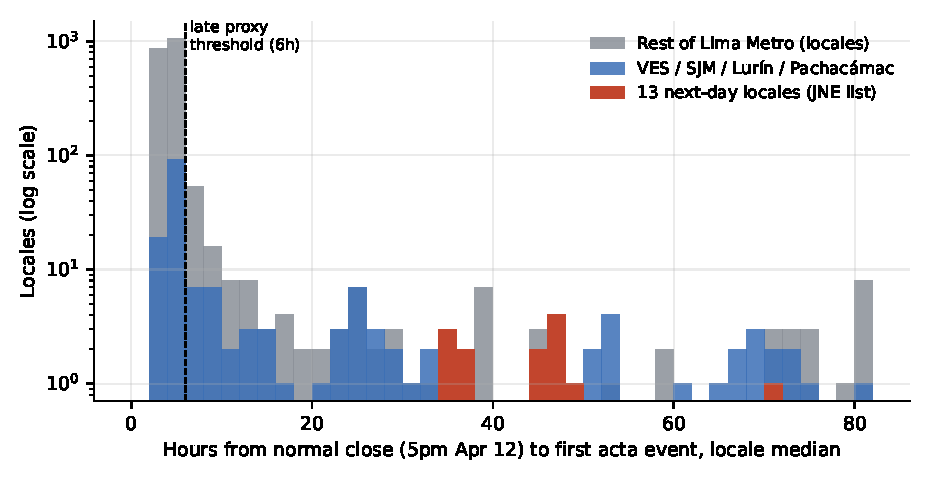
\includegraphics[width=.9\linewidth]{fig1_timing.pdf}
\caption{Locale-level timing of first acta transmission, Lima Metro. The 13 next-day locales (red) transmitted $\geq$22h after the normal close. The 6h threshold defines the late-opening proxy; locales from the four affected districts (blue) dominate the right tail.}
\label{fig:timing}
\end{figure}

\begin{table}[H]\centering\small
\caption{Analysis groups}
\begin{tabular}{lrrrrr}
\toprule
Group & Mesas & Locales & Registered & \shortstack{Turnout\\R1 (\%)} & \shortstack{Turnout\\R2 (\%)} \\
\midrule
Next-day mesas (13 locales, JNE list) & 187 & 13 & 55,261 & 75.3 & 81.1 \\
Late-locale proxy, 6h (excl.\ next-day) & 2,949 & 212 & 875,039 & 79.1 & 79.0 \\
Late-locale proxy, 12h (excl.\ next-day) & 1,508 & 119 & 447,242 & 79.2 & 79.6 \\
Rest of Lima Metro & 26,130 & 2,042 & 7,751,223 & 79.9 & 78.9 \\
Rest of Peru (domestic) & 60,957 & 8,060 & 17,433,096 & 73.4 & 71.5 \\
\bottomrule
\end{tabular}
\label{tab:desc}
\end{table}

\section{Empirical strategy}

For mesa $i$ in locale $\ell$, I estimate $y_{i} = \alpha + \beta\,T_{\ell} + \varepsilon_{i}$, with standard errors clustered by locale (treatment varies at the locale level). Following the requested comparisons, each treatment is estimated (1) against all other domestic mesas and (2) within Lima Metropolitana (province of Lima + Callao); I add (3) a specification with district fixed effects, and for the next-day treatment (4) a comparison restricted to the three affected districts. Late-proxy mesas are dropped from next-day regressions and vice versa, so controls are never contaminated by the other treatment. Because the next-day treatment has only 13 treated clusters, conventional cluster-robust inference is unreliable; I therefore also report randomization-inference $p$-values that re-assign the 13 treated locales within district (3/7/3 across SJM/Lurín/Pachacámac; 5,000 draws). Outcomes: votes cast and turnout (\% of registered), blank+null (\% of votes cast), the five leading candidates' shares of valid votes in round 1, the two runoff candidates' shares in round 2, and within-mesa changes across rounds (a mesa-level diff-in-diff that absorbs each mesa's electorate composition).

\section{Results}

\subsection{Next-day voting (the clean experiment)}

Table~\ref{tab:nextday} and Figures~\ref{fig:turnout}--\ref{fig:shares} summarize. Column (2) is the comparison ``vs.\ all others'' nationally; columns (3)--(5) progressively localize the counterfactual; column (6) reports RI $p$-values for the same-district comparison in column (5).

\begin{table}[t!]\centering\footnotesize
\caption{Effects of voting on April 13 (next-day mesas). SEs clustered by locale in parentheses. RI $p$-values from 5,000 within-district permutations of the 13 treated locales. *~$p<0.10$, **~$p<0.05$, ***~$p<0.01$.}
\begin{tabular}{lcccccc}
\toprule
 & \shortstack{Control\\mean} & National & Lima Metro & \shortstack{Lima Metro\\+ distr.\ FE} & \shortstack{3 affected\\districts} & \shortstack{RI\\$p$-value} \\
 & (1) & (2) & (3) & (4) & (5) & (6) \\
\midrule
\multicolumn{7}{l}{\emph{Panel A: First round}} \\
Registered voters (mesa size) & 298.0 & 6.33*** & -1.13 & -1.54 & -2.44 &  \\
 &  & (1.62) & (1.62) & (2.18) & (1.68) &  \\[1pt]
Turnout R1 (\%) & 80.2 & -0.11 & -4.66* & -5.68* & -4.91* & 0.019 \\
 &  & (2.41) & (2.41) & (2.98) & (2.52) &  \\[1pt]
Blank + null R1 (\% of cast) & 13.3 & -5.75*** & 0.42 & -1.92*** & -1.36*** & 0.013 \\
 &  & (0.30) & (0.31) & (0.62) & (0.43) &  \\[1pt]
Fujimori -- FP (\% valid) & 18.2 & 6.16*** & 5.80*** & 3.24*** & 5.36*** & 0.001 \\
 &  & (0.95) & (0.95) & (0.89) & (1.01) &  \\[1pt]
S\'anchez -- JP (\% valid) & 3.4 & -8.59*** & 3.57*** & 2.65*** & 2.96*** & 0.001 \\
 &  & (0.70) & (0.68) & (0.56) & (0.75) &  \\[1pt]
L\'opez Aliaga -- RP (\% valid) & 17.7 & 8.59*** & -1.33 & 3.24*** & 1.09 & 0.606 \\
 &  & (0.94) & (0.99) & (0.96) & (1.14) &  \\[1pt]
Nieto -- PBG (\% valid) & 14.5 & 21.41*** & 15.86*** & 17.07*** & 16.65*** & 0.000 \\
 &  & (0.84) & (0.85) & (1.08) & (0.95) &  \\[1pt]
Belmont -- Obras (\% valid) & 10.7 & -2.26*** & -0.94* & -3.08*** & -2.66*** & 0.000 \\
 &  & (0.51) & (0.52) & (0.57) & (0.67) &  \\[1pt]
\addlinespace
\multicolumn{7}{l}{\emph{Panel B: Second round}} \\
Turnout R2 (\%) & 79.9 & 7.38*** & 2.23 & 1.01 & 1.19 &  \\
 &  & (1.37) & (1.37) & (1.76) & (1.52) &  \\[1pt]
Blank + null R2 (\% of cast) & 6.3 & -0.79*** & -0.41** & -0.19 & -0.50** &  \\
 &  & (0.17) & (0.17) & (0.21) & (0.21) &  \\[1pt]
Fujimori -- FP, R2 (\% valid) & 62.5 & 12.97*** & -3.70*** & -2.01 & -1.54 &  \\
 &  & (1.41) & (1.40) & (1.39) & (1.61) &  \\[1pt]
S\'anchez -- JP, R2 (\% valid) & 37.5 & -12.97*** & 3.70*** & 2.01 & 1.54 &  \\
 &  & (1.41) & (1.40) & (1.39) & (1.61) &  \\[1pt]
\addlinespace
\multicolumn{7}{l}{\emph{Panel C: Within-mesa change}} \\
$\Delta$ Turnout (R2$-$R1) & -0.2 & 7.48*** & 6.89*** & 6.69** & 6.09*** & 0.000 \\
 &  & (1.96) & (1.96) & (2.72) & (1.99) &  \\[1pt]
$\Delta$ Blank + null (R2$-$R1) & -7.0 & 4.96*** & -0.82** & 1.74*** & 0.86* &  \\
 &  & (0.32) & (0.32) & (0.61) & (0.46) &  \\[1pt]
$\Delta$ Fujimori share (R2$-$R1) & 44.3 & 6.81*** & -9.50*** & -5.25*** & -6.89*** &  \\
 &  & (1.04) & (1.07) & (1.86) & (1.35) &  \\[1pt]
$\Delta$ S\'anchez share (R2$-$R1) & 34.1 & -4.38*** & 0.14 & -0.64 & -1.43 &  \\
 &  & (0.88) & (0.89) & (0.99) & (1.01) &  \\[1pt]
\addlinespace
\midrule
Observations &  & 87,274 & 26,317 & 26,317 & 988 &  \\
\bottomrule
\end{tabular}
\label{tab:nextday}
\end{table}

\begin{figure}[H]
\centering
\begin{minipage}{.44\linewidth}\centering
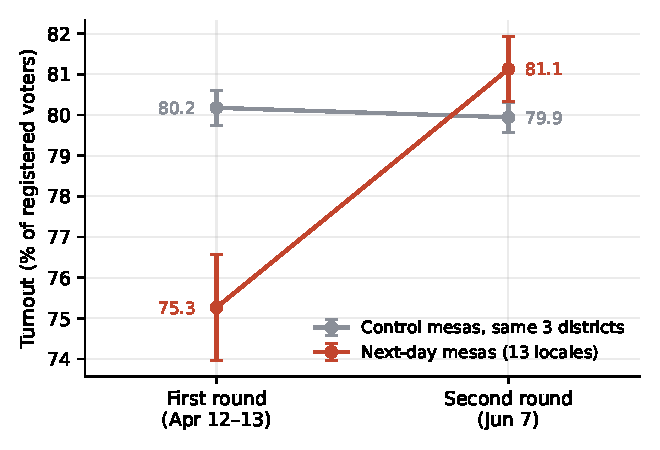
\includegraphics[width=\linewidth]{fig2_turnout.pdf}
\caption{Turnout by round: next-day mesas vs.\ control mesas in the same three districts.}
\label{fig:turnout}
\end{minipage}\hfill
\begin{minipage}{.53\linewidth}\centering
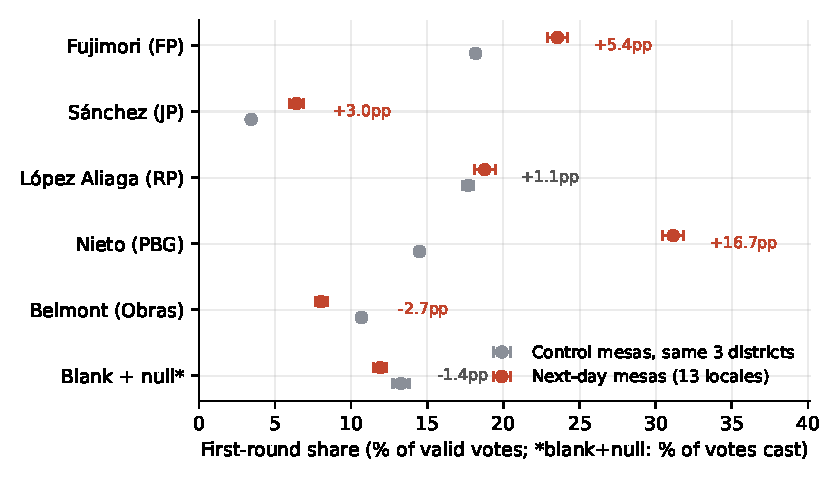
\includegraphics[width=\linewidth]{fig3_shares.pdf}
\caption{First-round outcomes, next-day vs.\ same-district control mesas (95\% CIs).}
\label{fig:shares}
\end{minipage}
\end{figure}

\textbf{Turnout.} Mesas voting on Monday lost $\approx$16 votes per mesa, or $-$4.7 to $-$5.7$\pp$ of turnout depending on the comparison (RI $p=0.019$)---from a control base of 80\%, i.e., $\sim$2,700 foregone votes across the 187 mesas. This closely matches DAL's $-$5$\pp$ estimate from actual installation times. Under compulsory voting with a fine, 94\% of the counterfactual electorate still showed up on a workday Monday; the intensive-margin damage was real but modest. Notably, mesa size (registered voters) is balanced across groups (column 5: $-$2.4, $p=0.15$), supporting the within-district comparison. \textbf{The dip was entirely transitory}: in the June runoff the same mesas turned out \emph{slightly above} their neighbors (+1.2$\pp$, n.s.), and the within-mesa change (Panel C) confirms a differential recovery of +6.1$\pp$ (RI $p<0.001$)---if anything suggesting mild re-mobilization rather than lasting disenfranchisement.

\textbf{Blank and invalid votes} fell by 1.4$\pp$ (RI $p=0.013$) from a base of 13.3\%. Monday's voters were a self-selected, better-informed group casting more deliberate ballots; mechanically, shorter queues and daylight scrutiny may also have reduced spoiled ballots.

\textbf{Vote shares (the headline result).} Monday voters, who knew the standings, voted very differently. Nieto (PBG), running fourth and 1.1$\pp$ from the runoff slot, jumped \textbf{+16.7$\pp$} over his 14.5\% same-district base (RI $p<0.001$)---more than doubling. Fujimori, the assured first-place finisher, gained +5.4$\pp$; S\'anchez +3.0$\pp$; Belmont, whose chances had evaporated, lost $-$2.7$\pp$; L\'opez Aliaga gained nothing (+1.1, RI $p=0.61$). The pattern is hard to reconcile with pure composition (why would Monday attrition disproportionately remove Belmont voters and add Nieto voters?) and looks like \emph{informed voting}: a bandwagon toward candidates seen as viable on Monday morning, away from those seen as finished. In the runoff the same mesas show only small, mostly insignificant differences (Panel B), consistent with a one-off information effect rather than persistent political idiosyncrasy of these locales.

\subsection{Late-opening locales (proxy)}

Effects are far smaller (Table~\ref{tab:late}). Within Lima Metro with district FE: turnout $-$0.8$\pp$ ($p=0.15$), blank+null +0.8$\pp$ ($p=0.001$), and small candidate-share effects (Fujimori +0.6$\pp$, S\'anchez +0.3$\pp$, L\'opez Aliaga $-$0.8$\pp$, Nieto $-$0.7$\pp$, all $p<0.10$). The within-mesa diff-in-diff corroborates a real but small turnout loss (treated mesas recovered +0.4 to +0.9$\pp$ more between rounds). The 12h proxy gives similar magnitudes. Two readings: (i) genuinely small effects---most late locales opened only a few hours late and voters could return during the day, and the fine kept them coming; (ii) attenuation from proxy misclassification (see \S\ref{sec:drawbacks}). Both surely operate; DAL's estimate with true opening times ($-$3$\pp$ for opening after 10am) suggests roughly two-thirds of the true effect is lost to measurement error in my proxy.

\begin{table}[t!]\centering\footnotesize
\caption{Effects at late-opening locales (transmission-timing proxy). SEs clustered by locale. Columns (2)--(3) use the 6h proxy; (4)--(5) the stricter 12h proxy. *~$p<0.10$, **~$p<0.05$, ***~$p<0.01$.}
\begin{tabular}{lcccccc}
\toprule
 & \shortstack{Control\\mean} & \shortstack{National\\(6h proxy)} & \shortstack{Lima Metro\\(6h proxy)} & \shortstack{Lima Metro\\+ distr.\ FE\\(6h proxy)} & \shortstack{Lima Metro\\(12h proxy)} & \shortstack{Lima Metro\\+ distr.\ FE\\(12h proxy)} \\
 & (1) & (2) & (3) & (4) & (5) & (6) \\
\midrule
\multicolumn{7}{l}{\emph{Panel A: First round}} \\
Registered voters (mesa size) & 296.6 & 7.54*** & 0.08 & -0.20 & -0.07 & -0.38 \\
 &  & (0.30) & (0.28) & (0.23) & (0.43) & (0.34) \\[1pt]
Turnout R1 (\%) & 79.9 & 3.74*** & -0.81 & -0.82 & -0.67 & -0.90 \\
 &  & (0.52) & (0.54) & (0.58) & (0.69) & (0.74) \\[1pt]
Blank + null R1 (\% of cast) & 11.5 & -5.45*** & 0.72** & 0.80*** & 1.40*** & 1.00*** \\
 &  & (0.33) & (0.33) & (0.24) & (0.43) & (0.32) \\[1pt]
Fujimori -- FP (\% valid) & 17.7 & 0.59 & 0.23 & 0.62** & 0.34 & 0.51 \\
 &  & (0.39) & (0.39) & (0.25) & (0.51) & (0.31) \\[1pt]
S\'anchez -- JP (\% valid) & 2.8 & -11.95*** & 0.20 & 0.32*** & 0.75*** & 0.47*** \\
 &  & (0.26) & (0.18) & (0.09) & (0.25) & (0.12) \\[1pt]
L\'opez Aliaga -- RP (\% valid) & 20.1 & 10.63*** & 0.72 & -0.76* & -0.90 & -1.35*** \\
 &  & (0.95) & (1.00) & (0.41) & (1.25) & (0.50) \\[1pt]
Nieto -- PBG (\% valid) & 15.3 & 5.56*** & 0.00 & -0.67** & -0.63 & -0.84** \\
 &  & (0.36) & (0.37) & (0.30) & (0.46) & (0.39) \\[1pt]
Belmont -- Obras (\% valid) & 9.0 & -1.44*** & -0.12 & 0.25* & 0.82* & 0.38** \\
 &  & (0.31) & (0.32) & (0.15) & (0.45) & (0.19) \\[1pt]
\addlinespace
\multicolumn{7}{l}{\emph{Panel B: Second round}} \\
Turnout R2 (\%) & 78.9 & 5.22*** & 0.07 & -0.44 & 0.75 & -0.28 \\
 &  & (0.52) & (0.54) & (0.57) & (0.67) & (0.71) \\[1pt]
Blank + null R2 (\% of cast) & 6.2 & -0.44*** & -0.06 & 0.09 & -0.20** & -0.04 \\
 &  & (0.07) & (0.07) & (0.08) & (0.10) & (0.10) \\[1pt]
Fujimori -- FP, R2 (\% valid) & 64.6 & 17.60*** & 0.93 & -0.59* & -1.05 & -1.38*** \\
 &  & (0.70) & (0.70) & (0.32) & (0.92) & (0.40) \\[1pt]
S\'anchez -- JP, R2 (\% valid) & 35.4 & -17.60*** & -0.93 & 0.59* & 1.05 & 1.38*** \\
 &  & (0.70) & (0.70) & (0.32) & (0.92) & (0.40) \\[1pt]
\addlinespace
\multicolumn{7}{l}{\emph{Panel C: Within-mesa change}} \\
$\Delta$ Turnout (R2$-$R1) & -1.0 & 1.48*** & 0.88*** & 0.38*** & 1.42*** & 0.62*** \\
 &  & (0.15) & (0.15) & (0.12) & (0.25) & (0.21) \\[1pt]
$\Delta$ Blank + null (R2$-$R1) & -5.3 & 5.00*** & -0.78** & -0.71*** & -1.60*** & -1.04*** \\
 &  & (0.31) & (0.31) & (0.24) & (0.41) & (0.32) \\[1pt]
$\Delta$ Fujimori share (R2$-$R1) & 46.9 & 17.02*** & 0.71 & -1.21*** & -1.39 & -1.90*** \\
 &  & (0.97) & (1.00) & (0.45) & (1.29) & (0.55) \\[1pt]
$\Delta$ S\'anchez share (R2$-$R1) & 32.5 & -5.66*** & -1.14** & 0.27 & 0.31 & 0.92*** \\
 &  & (0.54) & (0.55) & (0.27) & (0.72) & (0.34) \\[1pt]
\addlinespace
\midrule
Observations &  & 90,036 & 29,079 & 29,079 & 29,079 & 29,079 \\
\bottomrule
\end{tabular}
\label{tab:late}
\end{table}

\subsection{Could the delays have changed who made the runoff?}

The decisive margin was JP over RP by 21,210 votes. Combining the estimated share effects with the affected mesas' actual valid-vote totals: next-day mesas shifted the JP--RP margin by $\sim$+700 votes, late locales by $\sim$+6,600 (S\'anchez being helped, or at least not hurt, in both cases), and the turnout losses removed roughly 10,000 ballots that---even under extreme counterfactual allocations toward RP---could not plausibly span the gap. My estimates therefore agree with DAL's conclusion: the failures disenfranchised thousands and distorted choices at the margin, but are \emph{unlikely to have flipped the runoff slot}. Note the direction is awkward for the L\'opez Aliaga camp's legal claim: if anything, the delayed and next-day electorate broke toward S\'anchez and Nieto, not RP.

\section{Drawbacks of the proposed design}\label{sec:drawbacks}

\begin{enumerate}
\item \textbf{Treatment was not (quasi-)randomly assigned across Peru.} The premise of comparison ``vs.\ all others'' fails: one contractor's failure hit contiguous, mostly lower-income districts of Lima Sur. The national comparisons (column 2 of both tables) are dominated by \emph{Lima Sur vs.\ rest-of-country} differences---e.g., nationally the late proxy ``raises'' turnout by +3.7$\pp$ and ``lowers'' S\'anchez's share by 12$\pp$, both of which flip or vanish within Lima. Those columns should be read as descriptive only. The defensible designs are within-Lima, within-district (and, for candidate shares, the same-district column), where the identifying assumption---that \emph{which} locale in a district the truck failed to reach is as good as random---is plausible but untestable beyond the balance checks shown (mesa size balances; runoff outcomes barely differ).
\item \textbf{``Opened after 10am'' is not observable in these data.} The results files record acta processing, not installation. My locale-median transmission proxy (a) misses late-opening locales that still closed on time, (b) wrongly flags locales whose actas were merely processed late (e.g., JEE observation backlogs---note the flagged locales in Magdalena and San Miguel), and (c) inherits any correlation between processing backlogs and the chaos itself. Classification error at this scale plausibly attenuates effects by half or more. The fix is real opening times from the \emph{actas de instalación}: DAL has them (data by request), or we can OCR them ourselves---the JSONs contain every acta PDF's file ID.
\item \textbf{The April 13 ``treatment'' is a bundle.} Voting with results known combines (i) an information/strategic-voting effect, (ii) selection into who returns on a workday Monday, (iii) altered voting conditions (short queues, heavy JNE observation, media presence), and (iv) unchanged fine incentives. Turnout and blank+null effects mix (ii)--(iv); the share effects mix (i) with (ii). The Nieto/Fujimori/Belmont pattern strongly suggests (i) dominates, but with 187 mesas in 13 locales we cannot separate the channels. Worth saying plainly: this is an effect of \emph{voting after information release}, not a clean estimate of ``opening delay.''
\item \textbf{Spillovers onto the comparison group (SUTVA).} Same-district control locales sat amid the chaos: news coverage, crowds redirected, ONPE contingency efforts, and possible discouragement or mobilization of neighbors. If controls were partially treated, within-district estimates are biased toward zero; conversely the national estimates avoid spillover but import confounding. There is no design here that dodges both.
\item \textbf{Few treated clusters.} Thirteen treated locales make cluster-robust SEs anticonservative; I report randomization inference, which is the right benchmark here, but the effective sample for the next-day results is small and one or two idiosyncratic locales could move point estimates (Lurín contributes 7 of 13 treated locales and has only 3 untreated ones---its within-district counterfactual is thin).
\item \textbf{Post-treatment outcomes and endogenous acta handling.} Round-2 outcomes are measured \emph{after} treatment, so ``balance'' on them is suggestive, not proof. Also, actas from affected locales were more likely to be observed/challenged and to pass through JEE resolutions; if any votes were annulled differentially, measured shares partly reflect adjudication, not behavior.
\item \textbf{Compulsory voting compresses turnout responses.} With a fine ($\sim$S/.\ 100+, income-graded), the extensive margin is muted and the estimated $-$5$\pp$ is a lower bound on the disruption's behavioral push; external validity to voluntary-voting settings is limited. Relatedly, ``turnout'' here is votes cast at the mesa---anyone who gave up after seeing the chaos on Sunday but returned Monday is counted as voting, and there is no way to observe queue abandonment.
\item \textbf{Bundling blank with null.} Blank votes (nationally equal to 14\% of the R1 valid-vote total---more than every candidate but Fujimori!) are largely deliberate protest in this election, while null votes mix protest with error on a 5-contest ballot. Their determinants differ; I would report them separately in any paper version (the aggregate result here is driven by nulls at next-day mesas).
\item \textbf{Multiple testing.} Seventeen outcomes $\times$ several specifications: a few $p<0.10$ coefficients (e.g., the small candidate effects in the late-proxy FE column) should be discounted; the headline next-day results survive any sensible correction.
\end{enumerate}

\section{Suggested next steps}

(1) \textbf{Get real opening times}: request DAL's data (democracyactionlab@stanford.edu) or OCR the installation actas directly from the file IDs in our JSONs; then estimate dose--response in opening hour and replicate their after-10am cut. (2) \textbf{Exploit the runoff as a within-mesa counterfactual} more systematically (the Panel C DiD generalizes to a mesa-FE model pooling rounds). (3) \textbf{Congressional races}: the same mesas voted for Senate/Diputados on the same ballot; strategic-voting predictions differ sharply from the presidential race, giving a test of the information mechanism. (4) \textbf{Heterogeneity}: by district SES, mesa size, and distance to the nearest functioning locale. (5) \textbf{The two US next-day locales} (Paterson, Orlando) as out-of-Lima treated units. (6) \textbf{Exit-poll error decomposition}: Datum's erroneous quick count is itself an outcome of the chaos worth documenting. (7) If pursuing publication, engage with DAL early---their measurement is strictly better for the late-opening margin, but the next-day information-shock result and the runoff-recovery finding appear to be unexploited angles.

\vspace{1em}
\noindent\footnotesize\emph{Files: scripts and outputs in} \texttt{Dropbox/research projects/Claude/Elecciones 2026/} \emph{(01\_build\_dataset.py, 02\_regressions.do, 03\_permutation\_figures.py, 04\_make\_tables.py; mesa-level dataset in outputs/mesas\_analysis.dta). Sources: El Peruano, RPP, Diario Correo, Infobae, Expreso, TVPerú (April 12--13, 2026); Wikipedia ``Crisis postelectoral de Perú de 2026''; Democracy Action Lab, ``Missing Voters'' (cddrl-impactoelectoral.com).}

\end{document}
